\documentclass{beamer}
%
% Choose how your presentation looks.
%
% For more themes, color themes and font themes, see:
% http://deic.uab.es/~iblanes/beamer_gallery/index_by_theme.html
%
\mode<presentation>
{
  \usetheme{Madrid}      % or try Darmstadt, Madrid, Warsaw, ...
  \usecolortheme{seahorse} % or try albatross, beaver, crane, ...
  \usefonttheme{serif}  % or try serif, structurebold, ...
  \setbeamertemplate{navigation symbols}{}
  \setbeamertemplate{caption}[numbered]
} 

\usepackage[english]{babel}
\usepackage{kotex}
\usepackage{tikz}
\usepackage{listings}
\usepackage{pgffor}
\usepackage{listings}
\usepackage{amsfonts}
\usepackage[linesnumbered,ruled,vlined]{algorithm2e}
\usepackage{algorithmic}

% algorithmbis environment
\makeatletter
\newcounter{algorithmbis}[section]
\setcounter{algorithmbis}{0}
\renewcommand{\thealgorithmbis}{\arabic{algorithmbis}}
\def\algorithmbis{\@ifnextchar[{\@algorithmbisa}{\@algorithmbisb}}
\def\@algorithmbisa[#1]{%
  \refstepcounter{algorithmbis}
  \trivlist
  \leftmargin\z@
  \itemindent\z@
  \labelsep\z@
  \item[\colorbox{lightgray}{\parbox{\textwidth}{%
	    \noindent\strut\textbf{\sf\small 코드 \sf\small\thealgorithmbis} \sf\small#1}
  }]\hfil\vskip0em%
  \color{darkgray}
}
\def\@algorithmbisb{\@algorithmbisa[]}
\def\endalgorithmbis{\hfil\endtrivlist}
\makeatother

\lstset{ %
  backgroundcolor=\color{white},   % choose the background color; you must add \usepackage{color} or \usepackage{xcolor}
  basicstyle=\footnotesize,        % the size of the fonts that are used for the code
  breakatwhitespace=false,         % sets if automatic breaks should only happen at whitespace
  breaklines=true,                 % sets automatic line breaking
  captionpos=b,                    % sets the caption-position to bottom
  commentstyle=\color{gray},    % comment style
  deletekeywords={...},            % if you want to delete keywords from the given language
  escapeinside={\%*}{*)},          % if you want to add LaTeX within your code
  extendedchars=true,              % lets you use non-ASCII characters; for 8-bits encodings only, does not work with UTF-8
  frame=single,                    % adds a frame around the code
  keepspaces=true,                 % keeps spaces in text, useful for keeping indentation of code (possibly needs columns=flexible)
  keywordstyle=\color{blue},       % keyword style
  language=C++,                 % the language of the code
  morekeywords={*,...},            % if you want to add more keywords to the set
  numbers=left,                    % where to put the line-numbers; possible values are (none, left, right)
  numbersep=5pt,                   % how far the line-numbers are from the code
  numberstyle=\tiny\color{gray}, % the style that is used for the line-numbers
  rulecolor=\color{black},         % if not set, the frame-color may be changed on line-breaks within not-black text (e.g. comments (green here))
  showspaces=false,                % show spaces everywhere adding particular underscores; it overrides 'showstringspaces'
  showstringspaces=false,          % underline spaces within strings only
  showtabs=false,                  % show tabs within strings adding particular underscores
  stepnumber=1,                    % the step between two line-numbers. If it's 1, each line will be numbered
  stringstyle=\color{gray},     % string literal style
  tabsize=2,                       % sets default tabsize to 2 spaces
  title=\lstname                   % show the filename of files included with \lstinputlisting; also try caption instead of title
}

\title[3D 그래픽스 프로그래밍]{그래픽스 강의노트 03 - OpenGL 소개}
\author{강영민}
\institute{동명대학교}
\date{2015년 2학기}

\begin{document}

%%%%%%%%%%%%%%%%%%%%%%%%%%%%%%%%%%%%%%%%%%%%%%%%%%%%%%%%%
\begin{frame}
  \titlepage
\end{frame}

% Uncomment these lines for an automatically generated outline.
%\begin{frame}{Outline}
%  \tableofcontents
%\end{frame}


%%%%%%%%%%%%%%%%%%%%%%%%%%%%%%%%%%%%%%%%%%%%%%%%%%%%%%%%%%
%\begin{frame}[fragile]{깊이 버퍼와 이중 버퍼 사용 예제}
%   \lstset{language=C++,frame=none,escapechar=^}%
%    \foreach \n in {1,26,...,50} {%
%       \only<+>{%
%            \edef\m{\the\numexpr\n+24\relax}%
%            \edef\thesubtitle{{Lines \n--\m\ / 50}}%
%            \expandafter\framesubtitle\thesubtitle
%            \lstinputlisting[firstline=\n,lastline=\m]{./Codes/L03_depthAndDoubleBuffers.tex}%
%       }%
%    }
%\end{frame}
%%%%%%%%%%%%%%%%%%%%%%%%%%%%%%%%%%%%%%%%%%%%%%%%%%%%%%%%%%

%%%%%%%%%%%%%%%%%%%%%%%%%%%%%%%%%%%%%%%%%%%%%%%%%%%%%%%%%
%\begin{frame}[fragile]{간단한 OpenGL 프로그램 테스트}
%\lstset{language=C++,escapechar=^} 
%\begin{lstlisting}
%#include "headers.h"
%
%void myDisplay() {
%   glClear(GL_COLOR_BUFFER_BIT);
%    glFlush();    
%}
%\end{lstlisting}
%\end{frame}
%%%%%%%%%%%%%%%%%%%%%%%%%%%%%%%%%%%%%%%%%%%%%%%%%%%%%%%%%%


%%%%%%%%%%%%%%%%%%%%%%%%%%%%%%%%%%%%%%%%%%%%%%%%%%%%%%%%%
\begin{frame}[fragile]{OpenGL의 변환}

\begin{itemize}
\item 변환을 자유자재로 할 수 있다고 가정: $T( \mathbf p , \vec{d})$, 크기를 변경 $S( \mathbf p , s)$
\item 필요한 것은 반지름 1의 원 그리기 draw()만 있으면 어떤 위치에 어떤 크기로든 원을 그릴 수 있음
	\begin{itemize}
	\item $T ( S({\bf draw()}, s),  \vec{d})$
	\end{itemize}
\end{itemize}


\begin{itemize}
\item 어파인(affine) 변환 - 직선은 직선으로, 평행선은 평행선으로 유지
\end{itemize}

\begin{figure}
    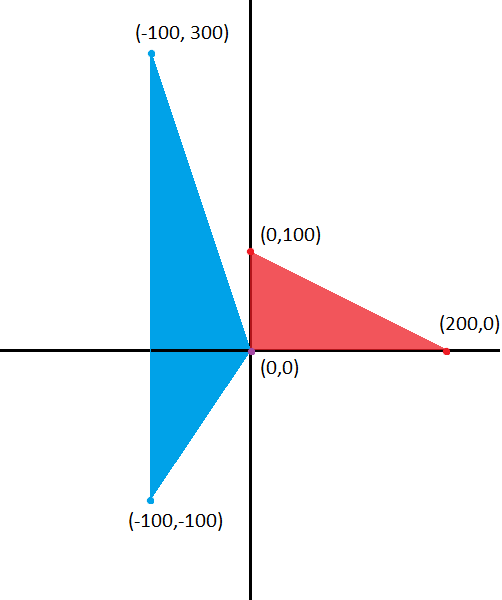
\includegraphics[height=5cm]{OGL_transform/affineXform.png}
\end{figure}

\end{frame}
%%%%%%%%%%%%%%%%%%%%%%%%%%%%%%%%%%%%%%%%%%%%%%%%%%%%%%%%%

%%%%%%%%%%%%%%%%%%%%%%%%%%%%%%%%%%%%%%%%%%%%%%%%%%%%%%%%%
\begin{frame}[fragile]{대표적인 어파인 변환}

\begin{table}
\label{tab:transform:affineXforms}
\begin{center}
    \begin{tabular}{ |l| p{7cm} |}
    \hline
    {이동(translate)} & {주어진 변위 벡터만큼 좌표를 동일하게 옮겨 놓는다.} \\[2em] \hline
    {회전(rotate)} & {2차원에서는 기준점, 3차원에서는 기준축을 중심으로 주어진 각도만큼 돌아간다.}\\[2em] \hline
    {크기변경(scale)} & {각 축 방향으로 주어진 비율에 따라 좌표 값이 커지거나 줄어든다.}\\[2em] \hline
    \hline
    \end{tabular}
\end{center}
\end{table}
\end{frame}
%%%%%%%%%%%%%%%%%%%%%%%%%%%%%%%%%%%%%%%%%%%%%%%%%%%%%%%%%

%%%%%%%%%%%%%%%%%%%%%%%%%%%%%%%%%%%%%%%%%%%%%%%%%%%%%%%%%
\begin{frame}[fragile]{동차좌표계}

\begin{itemize}
\item 동차 좌표(homogeneous coordinate)은 $n$ 차원의 사영공간을 $n+1$ 차원의 좌표로 나타내는 좌표계
\item 1827년 아우구스트 페르디난드 뫼비우스(August Ferdinand M\"{o}bius)가 그의 저작 ``Der barycentrische Cal\"{u}l"에서 처음으로 소개
\item 사영기하학에서 사용되는 좌표계
\item 무한의 위치에 있는 점을 유한 좌표로 표현하는 데에 적합
\end{itemize}

\begin{block}{그래픽스에서 동차좌표계를 사용하는 이유}
\begin{itemize}
\item 3차원 데카르트 좌표를 사용할 경우 이동은 벡터의 덧셈으로 표현되고, 회전은 $3 \times 3$ 행렬의 곱으로 표현
\item 이동과 회전이 누적되면 벡터 덧셈과 행렬 곱셈이 연속적 적용됨
\item 동차좌표(homogeneous coordinate)을 사용하면 이동과 회전 모두 $4 \times 4$ 행렬의 곱으로 표현 가능
\item 누적된 이동, 회전 변환을 하나의 행렬로 표현 가능
\end{itemize}
\end{block}

\end{frame}
%%%%%%%%%%%%%%%%%%%%%%%%%%%%%%%%%%%%%%%%%%%%%%%%%%%%%%%%%


%%%%%%%%%%%%%%%%%%%%%%%%%%%%%%%%%%%%%%%%%%%%%%%%%%%%%%%%%
\begin{frame}[fragile]{변환 행렬}

\begin{itemize}
\item 동차 좌표계에서 어파인 변환은 행렬로 표현
\item OpenGL 역시 변환을 행렬로 표현
\item OpenGL은 정점 데이터를 그래픽 카드로 보내는데, 각각의 정점들은 필요한 변환 행렬에 곱해져서 최종적인 화면 좌표 생성
\item 곱해지는 행렬은 두 종류: 모델뷰(ModelView) 행렬, 투영(Projection) 행렬
\item 하나의 정점이 화면 좌표로 바뀌는 과정
	\begin{itemize}
	\item 지역좌표계 내의 좌표를 $coord_{local}$이라고 하고, 모델뷰 행렬은 $ModelViewMatrix$, 투영행렬을 $ProjMatrix$라고 하면, 화면 좌표 $coord_{screen}$은 다음과 같이 구한다.
	\item $coord_{screen} = ProjMatrix  \times ModelViewMatrix \times coord_{local}$
	\end{itemize}
\end{itemize}

\end{frame}
%%%%%%%%%%%%%%%%%%%%%%%%%%%%%%%%%%%%%%%%%%%%%%%%%%%%%%%%%

%%%%%%%%%%%%%%%%%%%%%%%%%%%%%%%%%%%%%%%%%%%%%%%%%%%%%%%%%
\begin{frame}[fragile]{OpenGL에서 변환은 어떻게 이루어지나}

{\small
\begin{itemize}
\item OpenGL의 변환: $ModelViewMatrix$, $ProjMatrix$ 행렬을 변경하는 것
\item 모델 뷰 행렬, 투영 행렬 중 어는 것을 바꿀 것인지는 행렬 모드로 결정
\item 행렬모드: {\sf GL\_MODELVIEW}와 {\sf GL\_PROJECTION}  
	\begin{itemize}
	\item 당분간 {\sf GL\_TEXTURE}는 고려하지 않음
	\end{itemize}
\item 투영 행렬을 변경 = 카메라의 속성을 변경: {\sf glOrtho}나 {\sf gluPerspective}
\item 모델뷰 행렬을 변경하는 함수
	\begin{itemize}
	\item 카메라 위치 변경: {\sf gluLookAt}
	\item 객체의 위치, 방향, 크기 변경 - 표 참고
	\end{itemize}
\end{itemize}

    \begin{tabular}{ |l| p{7cm} |}
    \hline
    {\tiny \sf glTranslate3f(dx, dy, dz);} & {\tiny \sf (dx,dy,dz) 만큼 좌표 이동} \\ \hline
    {\tiny \sf glRotatef(angle, axisX, axisY, axisZ);} & {\tiny \sf 축(axisX, axisY, axisZ)를 기준으로 angle만큼 회전}\\ \hline
    {\tiny \sf glScalef(scaleX, scaleY, scaleZ);} & {\tiny \sf  (scaleX, scaleY, scaleZ)를 성분별로 좌표에 곱함}\\ \hline
    \hline
    \end{tabular}

\begin{itemize}
\item 이상의 변환들은 좌표를 변경하지 않고 행렬을 변경하는 역할을 수행
\item 현재의 행렬이 $\bf M$이라고 하고, {\sf glTranslate}의 이동을 표현하는 행렬이 $\bf T$
\item {\sf glTranslate} 함수가 불렸을 때, $\bf M$을 $\bf MT$로 변경
\end{itemize}
}

\end{frame}
%%%%%%%%%%%%%%%%%%%%%%%%%%%%%%%%%%%%%%%%%%%%%%%%%%%%%%%%%


%%%%%%%%%%%%%%%%%%%%%%%%%%%%%%%%%%%%%%%%%%%%%%%%%%%%%%%%%
\begin{frame}[fragile]{현재 변환 행렬}

\begin{itemize}
\item 현재 변환 행렬(current transform matrix)은 줄여서 CTM이라 부름
\item 모든 정점은 CTM에 곱해진다
\item 따라서 변환 함수는 이 CTM을 변경하는 것
\item CTM을 변경하는 함수로 다음과 같은 것들이 있다
\end{itemize}

\begin{tabular}{|c|p{7cm}|}\hline
{\small \sf 함수 } & {\small \sf CTM의 변경}\\ \hline
{\small \sf LoadIdentity} & {\small \sf CTM := I}\\ \hline
{\small \sf LoadMatrix(M)} & {\small \sf CTM := M}\\ \hline
{\small \sf T: Translate*} & {\small \sf CTM := CTM * T}\\ \hline
{\small \sf R: Rotate*} & {\small \sf CTM := CTM * R}\\ \hline
{\small \sf S: Scale*}	& {\small \sf CTM := CTM * S}\\ \hline
\end{tabular}

\end{frame}
%%%%%%%%%%%%%%%%%%%%%%%%%%%%%%%%%%%%%%%%%%%%%%%%%%%%%%%%%


%%%%%%%%%%%%%%%%%%%%%%%%%%%%%%%%%%%%%%%%%%%%%%%%%%%%%%%%%
\begin{frame}[fragile]{현재 변환 행렬}

\begin{itemize}
\item 현재 변환 행렬(current transform matrix)은 줄여서 CTM이라 부름
\item 모든 정점은 CTM에 곱해진다
\item 따라서 변환 함수는 이 CTM을 변경하는 것
\item CTM을 변경하는 함수로 다음과 같은 것들이 있다
\end{itemize}

\begin{tabular}{|c|p{7cm}|}\hline
{\small \sf 함수 } & {\small \sf CTM의 변경}\\ \hline
{\small \sf LoadIdentity} & {\small \sf CTM := I}\\ \hline
{\small \sf LoadMatrix(M)} & {\small \sf CTM := M}\\ \hline
{\small \sf T: Translate*} & {\small \sf CTM := CTM * T}\\ \hline
{\small \sf R: Rotate*} & {\small \sf CTM := CTM * R}\\ \hline
{\small \sf S: Scale*}	& {\small \sf CTM := CTM * S}\\ \hline
\end{tabular}

\end{frame}
%%%%%%%%%%%%%%%%%%%%%%%%%%%%%%%%%%%%%%%%%%%%%%%%%%%%%%%%%


%%%%%%%%%%%%%%%%%%%%%%%%%%%%%%%%%%%%%%%%%%%%%%%%%%%%%%%%%
\begin{frame}[fragile]{변환의 적용에 따른 CTM의 변화}

\begin{itemize}
\item 다음 코드와 같이 변환이 적용될 경우
\item CTM은 이 코드에 주석 처리된 부분에 나타난 것과 같이 변경
\end{itemize}

\lstset{language=C++, basicstyle=\small, escapechar=^} 
\begin{lstlisting}
glMatrixMode(GL_MODELVIEW);
glLoadIdentity();	// CTM:=I
glTranslatef(1,2,1);	// CTM:=IT ^{\it T는 glTranslate가 표현하는 행렬}^
glRotatef(45, 1,0,0);	// CTM:=ITR ^{\it R은 glRotate가 표현하는 행렬}^
glScalef(2.0, 1.0, 1.0);// CTM:=ITRS ^{\it S는 glScale이 표현하는 행렬}^
drawObjects();
\end{lstlisting}

\begin{block}{코드 구현 내용}
drawObjects 내에서 그려지는 모든 기하 객체의 좌표에 대해 크기변환($\mathbf S$)을 적용한 뒤, 이 값을 $x$ 축 기준으로 45도 회전하게 되며, 
이후 (1,2,1) 만큼의 이동을 한다. 다시말해 우리가 호출한 변환의 역순으로 변환이 객체에 적용된다.
\end{block}

\end{frame}
%%%%%%%%%%%%%%%%%%%%%%%%%%%%%%%%%%%%%%%%%%%%%%%%%%%%%%%%%

%%%%%%%%%%%%%%%%%%%%%%%%%%%%%%%%%%%%%%%%%%%%%%%%%%%%%%%%%
\begin{frame}[fragile]{구(sphere) 그리기에 변환 적용 예제}

\lstset{language=C++, escapechar=^} 
\begin{lstlisting}
void draw() {
    glutWireSphere(0.5, 30, 30); // ^{\it 반지름 0.5의 구를 원점을 중심으로 그림}^
}
void display() {
    ^{\sf [[여기에 카메라 설정(gluLookAt 등), 버퍼 클리어(glClear) 코드]]}^
    drawAxes(); // ^{\it 축을 그림}^
    glColor3f(1, 1, 0);
    draw(); // ^{\it 아무런 변환 없이 원점에 구를 그림}^
    glTranslatef(1.0, 0.0, 0.0); //^{\it $(1,0,0)$ 벡터만큼 이동을 함}^
    glColor3f(0, 1, 1);
    draw(); //^{\it 적용된 변환을 이용하여 구를 그림}^
    glTranslatef(-0.5, 1.0, 0.0); //^{\it $(-0.5,1,0)$ 벡터만큼 이동을 함}^
    glColor3f(1, 0, 0);
    draw(); //^{\it 적용된 변환을 이용하여 옮겨진 구를 그림}^
    glutSwapBuffers();
}
\end{lstlisting}

\end{frame}
%%%%%%%%%%%%%%%%%%%%%%%%%%%%%%%%%%%%%%%%%%%%%%%%%%%%%%%%%

%%%%%%%%%%%%%%%%%%%%%%%%%%%%%%%%%%%%%%%%%%%%%%%%%%%%%%%%%
\begin{frame}[fragile]{구(sphere) 그리기에 변환 적용 예제 실행 결과}

\begin{figure}
    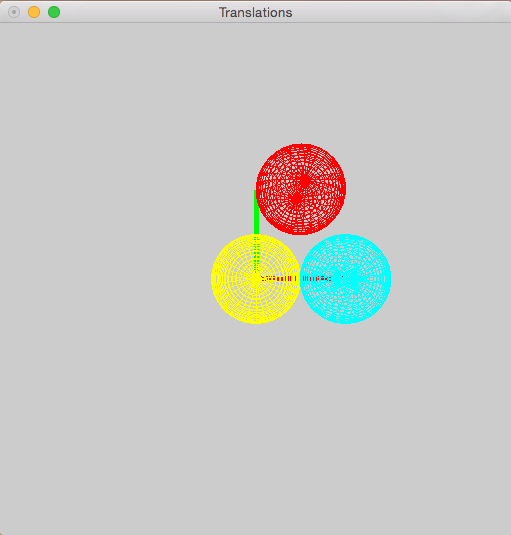
\includegraphics[height=4cm]{OGL_transform/transformedBalls.png}
\end{figure}

{\small
\begin{block}{}
\begin{itemize}
\item 노란 색, 하늘 색, 붉은 색 공이 차례로 그려진다.  
\item 노란 색 공에는 변환이 적용되지 않았으므로 원점에
\item 하늘 색 공에는 (1,1,0) 만큼의 이동
\item 붉은 색 공에 (-0.5, 1, 0) 적용 + 하늘 색에 적용된 (1,1,0) 이동이 추가
\end{itemize}
\end{block}
}

\end{frame}
%%%%%%%%%%%%%%%%%%%%%%%%%%%%%%%%%%%%%%%%%%%%%%%%%%%%%%%%%


%%%%%%%%%%%%%%%%%%%%%%%%%%%%%%%%%%%%%%%%%%%%%%%%%%%%%%%%%
\begin{frame}[fragile]{복합변환의 이해}

\begin{itemize}
\item 실제 객체에 적용되는 변환은 호출 순서의 역으로 적용
\item CTM을 활용한 변환 적용 기법을 사용하기 때문
\item 이러한 방식으로 이해하면 적용된 변환을 상상하기가 어려움
\item 다음 그림과 같이 네 개의 주전자를 배치하고 싶을 때에 OpenGL로 구현하려면 어떻게 해야할 지를 고민해 보자.
\end{itemize}

\begin{figure}
    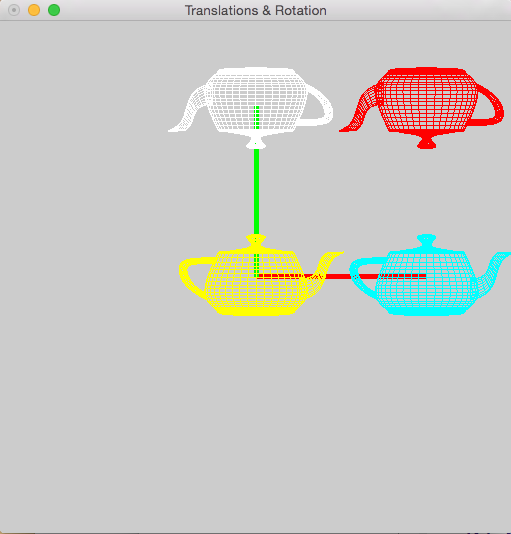
\includegraphics[height=5cm]{OGL_transform/fourTeapots.png}
\end{figure}


\end{frame}
%%%%%%%%%%%%%%%%%%%%%%%%%%%%%%%%%%%%%%%%%%%%%%%%%%%%%%%%%

%%%%%%%%%%%%%%%%%%%%%%%%%%%%%%%%%%%%%%%%%%%%%%%%%%%%%%%%%
\begin{frame}[fragile]{CTM 모델로 원하는 변환 구현해 보기}

{\small
\begin{itemize}
\item 노란색 주전자는 아무런 변환도 적용되지 않은 상태. 바로 그림
\end{itemize}
\lstset{language=C++, escapechar=^} 
\begin{lstlisting}
glLoadIdentity();
draw(yellow);				// CTM = I 
\end{lstlisting}

\begin{itemize}
\item 하늘색 주전자는 $x$ 축으로 1만큼 이동하여 그려야 하므로 {\sf glTranslate*} 함수를 부른 뒤 주전자를 그린다. 이 이동 변환을 T1이라고 하자.
\end{itemize}
\lstset{language=C++, escapechar=^} 
\begin{lstlisting}
glTranslatef(1.0, 0.0, 0.0);  // T1
draw(cyan);
\end{lstlisting}

\begin{itemize}
\item 붉은 주전자는 $z$ 축을 기준으로 180도 회전한 뒤에 (1,1,0)만큼 이동
\item 현재의 CTM이 ${\mathbf T}_1$이므로 (0,1,0)만큼의 이동 ${\mathbf T}_2$를 추가 적용하면 (1,1,0) 이동이 되며, 여기에 회전 ${\mathbf R}$을 적용
\end{itemize}
\lstset{language=C++, escapechar=^} 
\begin{lstlisting}
glTranslate(0.0, 1.0, 0.0);		// T2
glRotatef(180, 0.0, 0.0, 1.0);	// R
draw(red);
\end{lstlisting}
}
\end{frame}
%%%%%%%%%%%%%%%%%%%%%%%%%%%%%%%%%%%%%%%%%%%%%%%%%%%%%%%%%

%%%%%%%%%%%%%%%%%%%%%%%%%%%%%%%%%%%%%%%%%%%%%%%%%%%%%%%%%
\begin{frame}[fragile]{CTM 모델로 원하는 변환 구현해 보기}

{\small

\begin{itemize}
\item 붉은 색 주전자는 ${\mathbf T}_1 {\mathbf T}_2  {\mathbf R}$의 변환
\item 흰색 주전자를 그리는 방법은 까다롭다
\item 이 주전자는 180도 회전 시킨 주전자를 (0,1,0) 만큼 이동한 것
\item 현재의 변환 ${\mathbf T}_1 {\mathbf T}_2  {\mathbf R}$에 어떤 변환을 추가적으로 호출하면 이것이 가능할지 생각해야 함
\item 회전이 호출된 상태라 까다롭다.
\item 새롭게 적용할 변환이 $\mathbf  X$라고 하고, (0,1,0) 만큼 이동하는 변환을 ${\mathbf T}$라고 하면 다음과 같은 관계 성립
	\begin{itemize}
	\item ${\mathbf T_1 \mathbf T_2 \mathbf R \mathbf X } = {\mathbf T \mathbf R} $
	\item $ {\mathbf X} = { \mathbf R^T {\mathbf T_2}^{-1} {\mathbf T_1}^{-1} \mathbf T \mathbf R}$
	\end{itemize}
\item 위의 계산을 수행하면 X는 (1,0,0) 만큼의 이동으로 나타나게 된다. 따라서 다음과 같이 적용하면 원하는 결과를 얻을 수 있다.
\end{itemize}

\begin{verbatim}
glTranslatef(1.0, 0.0, 0.0);	// X
draw(white);
\end{verbatim}

}
\end{frame}
%%%%%%%%%%%%%%%%%%%%%%%%%%%%%%%%%%%%%%%%%%%%%%%%%%%%%%%%%


%%%%%%%%%%%%%%%%%%%%%%%%%%%%%%%%%%%%%%%%%%%%%%%%%%%%%%%%%
\begin{frame}[fragile]{지역 좌표계 변환을 중심으로 생각하기 1/6}

\begin{itemize}
\item 앞 슬라이드의 방식은 너무 번거롭다.
\item 쉬운 방법: 물체의 변환이 아니라 좌표계의 변환으로 이해
\item 각각의 주전자가 가진 지역 좌표계를 함께 그리기
\item 노란색 주전자는 변환 적용 없어 전역 좌표계와 일치
\end{itemize}

\begin{figure}
    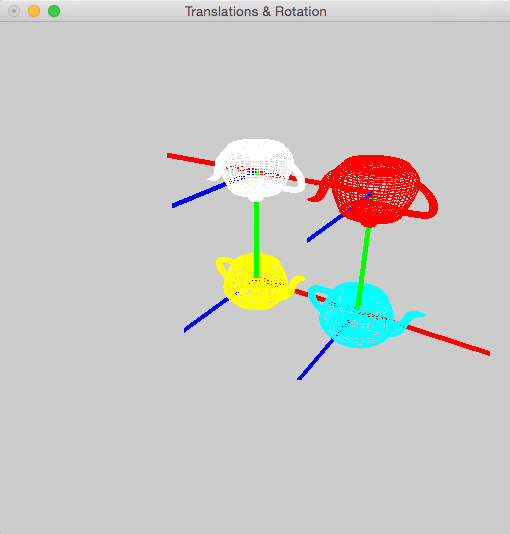
\includegraphics[height=4.5cm]{OGL_transform/localCoordXform.png}
\end{figure}

\begin{verbatim}
glLoadIdentity();
draw(yellow);
\end{verbatim}

\end{frame}
%%%%%%%%%%%%%%%%%%%%%%%%%%%%%%%%%%%%%%%%%%%%%%%%%%%%%%%%%


%%%%%%%%%%%%%%%%%%%%%%%%%%%%%%%%%%%%%%%%%%%%%%%%%%%%%%%%%
\begin{frame}[fragile]{지역 좌표계 변환을 중심으로 생각하기 2/6}

\begin{figure}
    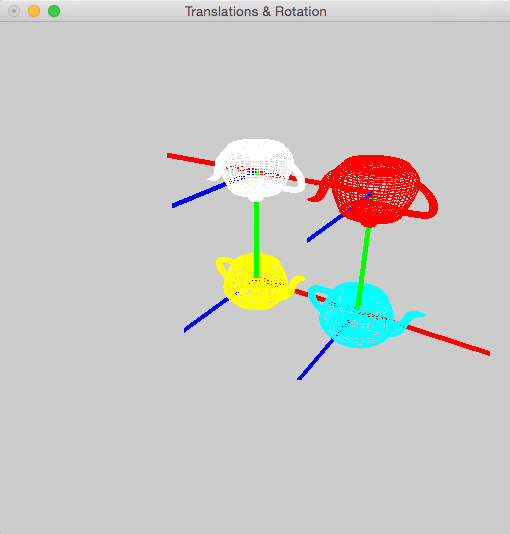
\includegraphics[height=4.5cm]{OGL_transform/localCoordXform.png}
\end{figure}

하늘색 주전자는 노란색 주전자의 좌표계에서 보았을 때 $x$ 축으로 1만큼 이동하여 있다. 따라서 다음과 같이 적용한다.

\begin{verbatim}
glTranslatef(1.0,0.0,0.0);
draw(cyan);
\end{verbatim}

\end{frame}
%%%%%%%%%%%%%%%%%%%%%%%%%%%%%%%%%%%%%%%%%%%%%%%%%%%%%%%%%

%%%%%%%%%%%%%%%%%%%%%%%%%%%%%%%%%%%%%%%%%%%%%%%%%%%%%%%%%
\begin{frame}[fragile]{지역 좌표계 변환을 중심으로 생각하기 3/6}

\begin{figure}
    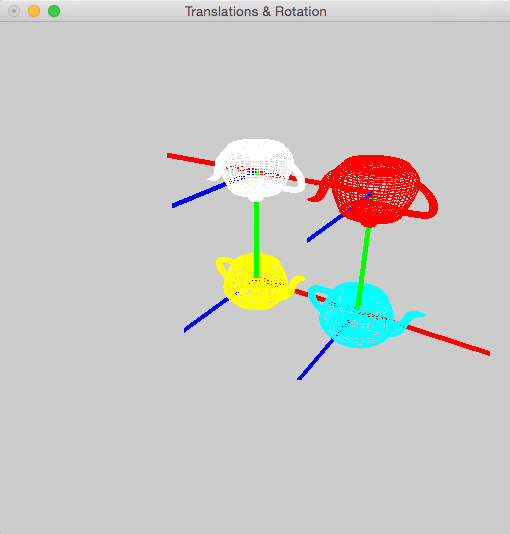
\includegraphics[height=4.5cm]{OGL_transform/localCoordXform.png}
\end{figure}

붉은 색 주전자는 하늘색 주전자에서 $y$ 축으로 1만큼 올라간 뒤에, {\bf 이동된 좌표계}에서 $z$축을 기준으로 180도 회전

\begin{verbatim}
glTranslatef(0.0, 1.0, 0.0);
glRotatef(180, 0.0, 0.0, 1.0);
draw(red);
\end{verbatim}

\end{frame}
%%%%%%%%%%%%%%%%%%%%%%%%%%%%%%%%%%%%%%%%%%%%%%%%%%%%%%%%%

%%%%%%%%%%%%%%%%%%%%%%%%%%%%%%%%%%%%%%%%%%%%%%%%%%%%%%%%%
\begin{frame}[fragile]{지역 좌표계 변환을 중심으로 생각하기 4/6}

\begin{figure}
    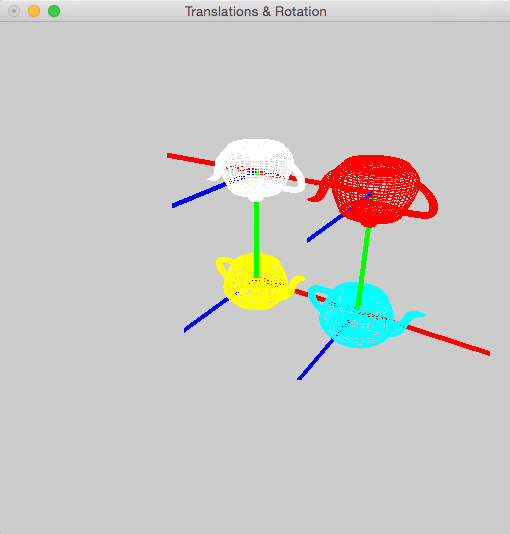
\includegraphics[height=4.5cm]{OGL_transform/localCoordXform.png}
\end{figure}

붉은 주전자의 변환은 순서를 바꾸어 하늘색 주전자에서 $z$축 회전을 먼저 적용한 뒤에 
$y$축 기준으로 -1만큼 이동하는 것과도 같다. 따라서 다음과 같이 적용해도 동일한 결과

\begin{verbatim}
glRotatef(180, 0.0, 0.0, 1.0);
glTranslatef(0.0, -1.0, 0.0);
draw(red);
\end{verbatim}

\end{frame}
%%%%%%%%%%%%%%%%%%%%%%%%%%%%%%%%%%%%%%%%%%%%%%%%%%%%%%%%%

%%%%%%%%%%%%%%%%%%%%%%%%%%%%%%%%%%%%%%%%%%%%%%%%%%%%%%%%%
\begin{frame}[fragile]{지역 좌표계 변환을 중심으로 생각하기 5/6}

\begin{figure}
    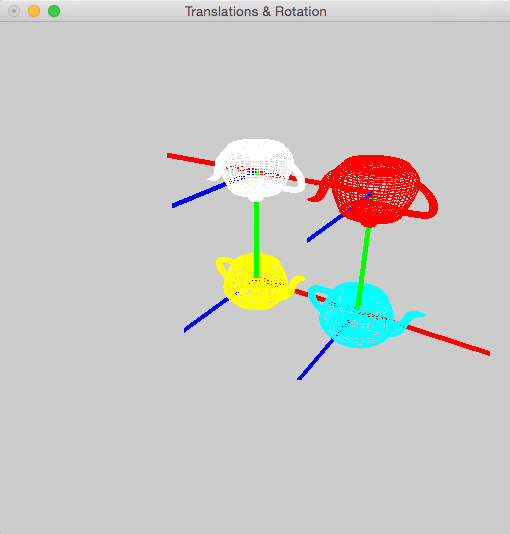
\includegraphics[height=4.5cm]{OGL_transform/localCoordXform.png}
\end{figure}

마지막으로 흰색 주전자는 붉은 색 주전자에서 $x$ 축으로 1만큼 이동한 것

\begin{verbatim}
glTranslatef(1.0, 0.0, 0.0);
draw(white);
\end{verbatim}

\end{frame}
%%%%%%%%%%%%%%%%%%%%%%%%%%%%%%%%%%%%%%%%%%%%%%%%%%%%%%%%%

%%%%%%%%%%%%%%%%%%%%%%%%%%%%%%%%%%%%%%%%%%%%%%%%%%%%%%%%%
\begin{frame}[fragile]{지역 좌표계 변환을 중심으로 생각하기 6/6}

\lstset{language=C++, escapechar=^} 
\begin{lstlisting}
void drawLocalAxes() { drawAxes(); }
void draw() {    glutWireTeapot(0.3);}

void display() {

    ^{\sf [[카메라 설정과 버퍼 지우기 등의 코드]]}^

    drawLocalAxes();
    glColor4f(1, 1, 0, 0.25);
    draw();
    
    glTranslatef(1.0, 0.0, 0.0);
    drawLocalAxes();
    glColor4f(0, 1, 1, 0.25);
    draw();
    
    glRotatef(180, 0.0, 0.0, 1.0);
    glTranslatef(0.0,-1.0, 0.0);
    drawLocalAxes();
    glColor4f(1, 0, 0, 0.25);
    draw();
    
    glTranslatef(1.0, 0.0, 0.0);
    drawLocalAxes();
    glColor4f(1, 1, 1, 0.25);
    draw();
    
    glutSwapBuffers();
}

\end{lstlisting}

\end{frame}
%%%%%%%%%%%%%%%%%%%%%%%%%%%%%%%%%%%%%%%%%%%%%%%%%%%%%%%%%

%%%%%%%%%%%%%%%%%%%%%%%%%%%%%%%%%%%%%%%%%%%%%%%%%%%%%%%%%
\begin{frame}[fragile]{크기 변경이 포함된 경우}

{\small
\begin{itemize}
\item 크기 변경이 포함될 경우에는 문제가 발생
	\begin{itemize}
	\item 지역좌표계 변환을 통한이해는 강체(rigid) 변환에 대해서만 적용
	\end{itemize}
\item 다음의 그림과 같은 장면을 그린다고 가정
	\begin{itemize}
	\item 각 변 길이 1인 정육면체를 높이 2, 너비 1, 깊이 1로 만들 경우
	\item glScalef(1.0, 2.0, 1.0);
	\end{itemize}
\end{itemize}
}
\begin{figure}
    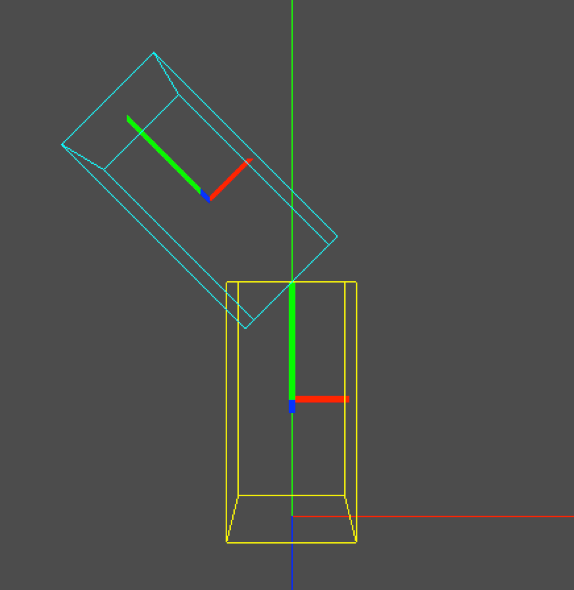
\includegraphics[height=5cm]{OGL_transform/noScale.png}
\end{figure}

\end{frame}
%%%%%%%%%%%%%%%%%%%%%%%%%%%%%%%%%%%%%%%%%%%%%%%%%%%%%%%%%

%%%%%%%%%%%%%%%%%%%%%%%%%%%%%%%%%%%%%%%%%%%%%%%%%%%%%%%%%
\begin{frame}[fragile]{크기 변경이 포함된 경우}

\begin{itemize}
\item 육면체가 $xz$ 평면위에 놓이려면 $y$축 방향으로 0.5 이동
	\begin{itemize}
	\item 이미 지역좌표계가 {\sf glScale}에 의해 변환되었기 때문에 0.5만 들어올려도 전역좌표계에서는 1만큼 올라가게 된다.
	\end{itemize}
\item 노란색 육면체는 다음과 같이 그림
\end{itemize}

\lstset{language=C++, escapechar=^} 
\begin{lstlisting}
glScalef(1.0, 2.0, 1.0);		// S
glTranslatef(0.0, 0.5, 0.0);	// T1
draw(yellow);
\end{lstlisting}


\begin{itemize}
\item 문제는 하늘색 육면체
\item 이 육면체는 노란색 육면체를 0.5만큼 들어올린 뒤에 z축 기준으로 회전을 시키고, 이렇게 변환된 공간에서 다시 y축 기준으로 0.5만큼 이동시키면 됨
\item 코드로는 다음과 같은 변환 적용으로 구현이 가능할 것처럼 보임
\end{itemize}

\lstset{language=C++, escapechar=^} 
\begin{lstlisting}
glTranslatef(0.0, 0.5, 0.0);	// T2
glRotatef(45, 0.0, 0.0, 1.0);	// R
glTranslatef(0.0, 0.5, 0.0);	// T3
draw(cyan);
\end{lstlisting}

\end{frame}
%%%%%%%%%%%%%%%%%%%%%%%%%%%%%%%%%%%%%%%%%%%%%%%%%%%%%%%%%

%%%%%%%%%%%%%%%%%%%%%%%%%%%%%%%%%%%%%%%%%%%%%%%%%%%%%%%%%
\begin{frame}[fragile]{크기 변경이 포함된 경우}

결과는...

\begin{figure}
    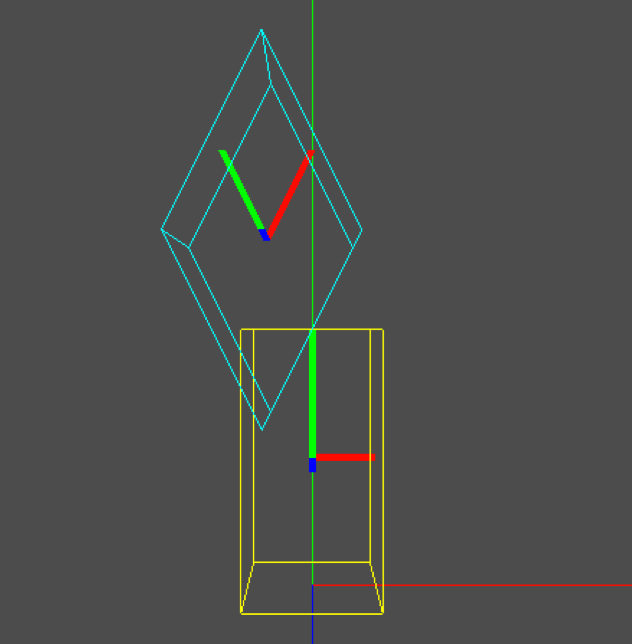
\includegraphics[height=7cm]{OGL_transform/scale.png}
\end{figure}

\end{frame}
%%%%%%%%%%%%%%%%%%%%%%%%%%%%%%%%%%%%%%%%%%%%%%%%%%%%%%%%%

%%%%%%%%%%%%%%%%%%%%%%%%%%%%%%%%%%%%%%%%%%%%%%%%%%%%%%%%%
\begin{frame}[fragile]{크기 변경이 포함된 경우}

\begin{itemize}
\item 실제로 하늘색 육면체에 적용된 변환
\item ${\mathbf S \mathbf T_1 \mathbf T_2 \mathbf R \mathbf T_3}$
\item 가장 마지막에 적용되는 ${\mathbf S}$는 전역 좌표계를 기준으로 크기변경
\item 하늘색 육면체의 방향(orientation)을 고려하지 않고 크기 변경
\item 해결하는 방법은 행렬 스택 연산인 {\sf glPushMatrix()}와 {\sf glPopMatrix()}를 활용하여 크기변경 변환은 적용된 객체 이외에서 영향을 미치지 않도록 제한
\end{itemize}

\begin{center}
\begin{tabular}{|c|p{7cm}|}\hline
{\small \sf 함수명} & {\small \sf 역할}\\ \hline
{\small \sf glPushMatrix} & {\small \sf 현재의 CTM을 스택에 저장한다.}\\ \hline
{\small \sf glPopMatrix} & {\small \sf 행렬 스택을 pop하여 CTM을 갱신한다.}\\ \hline
\end{tabular}
\end{center}

\begin{itemize}
\item {\sf glPushMatrix}를 수행한 뒤에 {\sf glPopMatrix}를 수행하면 직전의 {\sf glPushMatrix} 수행 당시의 CTM으로 복원
\end{itemize}

\end{frame}
%%%%%%%%%%%%%%%%%%%%%%%%%%%%%%%%%%%%%%%%%%%%%%%%%%%%%%%%%

%%%%%%%%%%%%%%%%%%%%%%%%%%%%%%%%%%%%%%%%%%%%%%%%%%%%%%%%%
\begin{frame}[fragile]{크기 변경이 포함된 경우}

\lstset{language=C++, escapechar=^} 
\begin{lstlisting}
glTranslatef(0.0, 1.0, 0.0);
glPushMatrix();
glScalef(1.0, 2.0, 1.0);
draw(yellow);
glPopMatrix();

glTranslatef(0.0, 1.0, 0.0);
glRotatef(45, 0.0, 0.0, 0.0);
glTranslatef(0.0, 1.0, 0.0);
glPushMatrix();
glScalef(1.0, 2.0, 1.0);
draw(cyan);
glPopMatrix();
\end{lstlisting}

\begin{figure}
    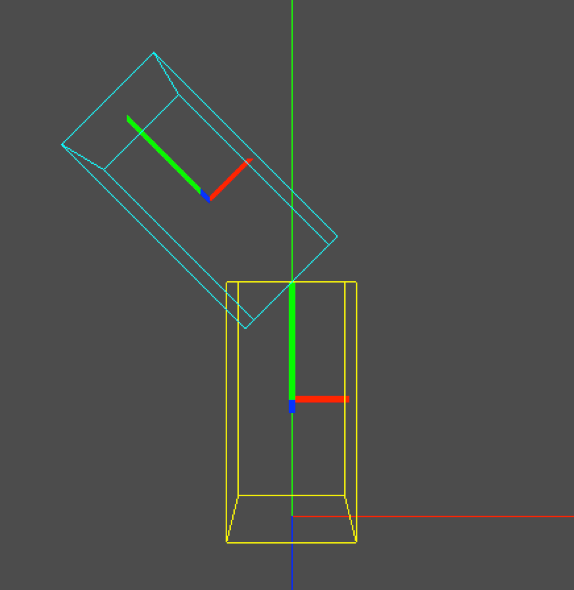
\includegraphics[height=3cm]{OGL_transform/noScale.png}
\end{figure}

\end{frame}
%%%%%%%%%%%%%%%%%%%%%%%%%%%%%%%%%%%%%%%%%%%%%%%%%%%%%%%%%


%%%%%%%%%%%%%%%%%%%%%%%%%%%%%%%%%%%%%%%%%%%%%%%%%%%%%%%%%
\begin{frame}[fragile]{계층적 구조}

\begin{itemize}
\item 컴퓨터 그래픽스로 표현하는 객체: 구조를 가짐
\item 많은 경우 이 구조는 인간이나 로봇과 같은 구조체에서 볼 수 있는 바와 같이 계층적(hierarchical) 
\end{itemize}

\begin{figure}
    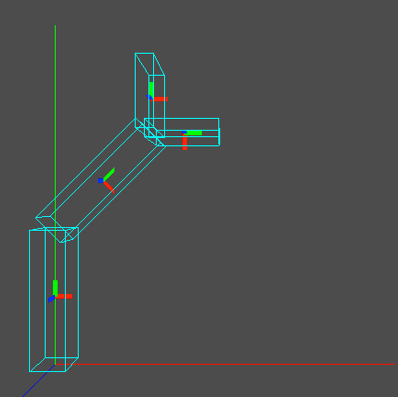
\includegraphics[height=5cm]{OGL_transform/robotArm.png}
\end{figure}

\end{frame}
%%%%%%%%%%%%%%%%%%%%%%%%%%%%%%%%%%%%%%%%%%%%%%%%%%%%%%%%%

%%%%%%%%%%%%%%%%%%%%%%%%%%%%%%%%%%%%%%%%%%%%%%%%%%%%%%%%%
\begin{frame}[fragile]{계층적 모델링(hierarchical modeling) 1/2}

\begin{itemize}
\item 계층적 모델링은 앞서 살펴본 {\sf glPushMatrix}와 {\sf glPopMatrix}를 활용하여 구현
\item 팔 구성 요소는 길이가 4이며, 손을 구성하는 요소는 길이가 2라고 가정
\item 팔 구성요소를 그리는 함수를 {\sf drawArm()}이라 하자.
\item 손을 그리는 함수는 {\sf drawHand()}
\item 루트(root) 객체인 가장 아래쪽 육면체는 팔 요소의 길이 4를 고려하여 그 반에 해당하는 2만큼 위로 올림
	\begin{itemize}
	\item glTranslatef(0.0, 2.0, 0.0);
	\item drawArm();
	\end{itemize}
\item 다음으로 45$^{\circ}$로 누워 있는 팔은 부모 노드의 변환을 반영해야 하므로 앞서 적용된 변환을 유지한 상태로 팔의 길이의 반만큼 올라간 뒤, 45도 회전하고, 나머지 반을 더 올라가서 끝을 맞춤
	\begin{itemize}
	\item glTranslatef(0.0, 2.0, 0.0);
	\item glRotatef(-45, 0.0, 0.0, 1.0);
	\item glTranslatef(0.0, 2.0, 0.0);
	\item drawArm();
	\end{itemize}
\end{itemize}
\end{frame}
%%%%%%%%%%%%%%%%%%%%%%%%%%%%%%%%%%%%%%%%%%%%%%%%%%%%%%%%%

%%%%%%%%%%%%%%%%%%%%%%%%%%%%%%%%%%%%%%%%%%%%%%%%%%%%%%%%%
\begin{frame}[fragile]{계층적 모델링(hierarchical modeling) 2/2}

\begin{itemize}
\item 손의 중심을 팔의 끝에 두기 위해 팔의 길이 반에 해당하는 2만큼 이동시킨뒤 45$^{\circ}$ 회전하고, 손의 끝점을 관절부에 맞추기 위해 손의 길이 2의 반인 1만큼 이동하여 그림
\item 두 번째 손을 그리려면 이 변환은 무효화되어야 함
\item glPushMatrix를 이용하여 현재의 변환을 기록했다가 다시 복원
	\begin{itemize}
	\item glPushMatrix();
	\item glTranslatef(0.0, 2.0, 0.0); 
	\item glRotatef(-45, 0.0, 0.0, 1.0);
	\item glTranslatef(0.0, 1.0, 0.0);
	\item glPopMatrix();
	\end{itemize}
\item 다음으로 마지막 손 요소를 그림
	\begin{itemize}
	\item glTranslatef(0.0, 2.0, 0.0); 
	\item glRotatef(45, 0.0, 0.0, 1.0);
	\item glTranslatef(0.0, 1.0, 0.0);
	\end{itemize}
\end{itemize}


\end{frame}
%%%%%%%%%%%%%%%%%%%%%%%%%%%%%%%%%%%%%%%%%%%%%%%%%%%%%%%%%

%%%%%%%%%%%%%%%%%%%%%%%%%%%%%%%%%%%%%%%%%%%%%%%%%%%%%%%%%
\begin{frame}[fragile]{로봇 팔 그리기 예제}
   \lstset{language=C++,frame=none,escapechar=^}%
    \foreach \n in {1,26,...,50} {%
       \only<+>{%
            \edef\m{\the\numexpr\n+24\relax}%
            \edef\thesubtitle{{Lines \n--\m\ / 50}}%
            \expandafter\framesubtitle\thesubtitle
            \lstinputlisting[firstline=\n,lastline=\m]{./Codes/L04_robotArm.tex}%
       }%
    }
\end{frame}
%%%%%%%%%%%%%%%%%%%%%%%%%%%%%%%%%%%%%%%%%%%%%%%%%%%%%%%%%

%%%%%%%%%%%%%%%%%%%%%%%%%%%%%%%%%%%%%%%%%%%%%%%%%%%%%%%%%
\begin{frame}[fragile]{가상의 태양계 그리기}
   \lstset{language=C++,frame=none,escapechar=^}%
    \foreach \n in {1,26,...,75} {%
       \only<+>{%
            \edef\m{\the\numexpr\n+24\relax}%
            \edef\thesubtitle{{Lines \n--\m\ / 75}}%
            \expandafter\framesubtitle\thesubtitle
            \lstinputlisting[firstline=\n,lastline=\m]{./Codes/L04_solarSystem.tex}%
       }%
    }
\end{frame}
%%%%%%%%%%%%%%%%%%%%%%%%%%%%%%%%%%%%%%%%%%%%%%%%%%%%%%%%%

%%%%%%%%%%%%%%%%%%%%%%%%%%%%%%%%%%%%%%%%%%%%%%%%%%%%%%%%%
\begin{frame}[fragile]{가상의 태양계 그리기}

\begin{figure}
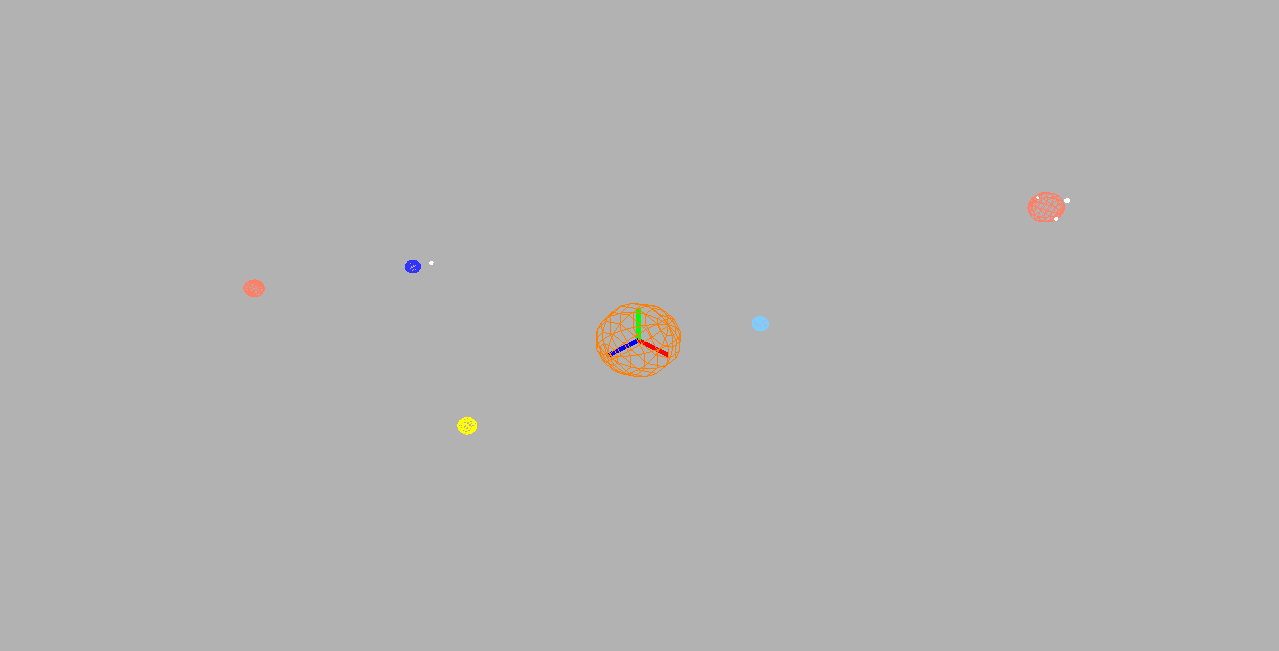
\includegraphics[height=6cm]{OGL_transform/solar1.png}
\end{figure}

\end{frame}
%%%%%%%%%%%%%%%%%%%%%%%%%%%%%%%%%%%%%%%%%%%%%%%%%%%%%%%%%


%%%%%%%%%%%%%%%%%%%%%%%%%%%%%%%%%%%%%%%%%%%%%%%%%%%%%%%%%
\begin{frame}[fragile]{궤도 그려 넣기}

\begin{itemize}
\item 각 천체들이 움직이는 공전궤도를 표현하고 싶다면
\item 공전 궤도를 표현할 drawCircle(radius)  함수를 다음과 같이 구현
\end{itemize}

\lstset{language=C++} 
\begin{lstlisting}
void drawCircle(float radius) {
   glColor3f(1.0, 1.0, 1.0);
   glBegin(GL_LINE_LOOP);
   for (int i=0; i<50; i++) {
     glVertex3f(
            radius*cos(6.28*float(i)/50.0), 
            0.0, 
            radius*sin(6.28*float(i)/50.0));
   }
   glEnd();
}
\end{lstlisting}

\begin{itemize}
\item 이제 이 drawCircle 함수를 어디에서 부를 것인지를 결정
\end{itemize}

\end{frame}
%%%%%%%%%%%%%%%%%%%%%%%%%%%%%%%%%%%%%%%%%%%%%%%%%%%%%%%%%

%%%%%%%%%%%%%%%%%%%%%%%%%%%%%%%%%%%%%%%%%%%%%%%%%%%%%%%%%
\begin{frame}[fragile]{궤도 그려 넣기}
   \lstset{language=C++,frame=none,escapechar=^}%
    \foreach \n in {1,26,...,50} {%
       \only<+>{%
            \edef\m{\the\numexpr\n+24\relax}%
            \edef\thesubtitle{{Lines \n--\m\ / 50}}%
            \expandafter\framesubtitle\thesubtitle
            \lstinputlisting[firstline=\n,lastline=\m]{./Codes/L04_solarSystem2.tex}%
       }%
    }
\end{frame}
%%%%%%%%%%%%%%%%%%%%%%%%%%%%%%%%%%%%%%%%%%%%%%%%%%%%%%%%%

%%%%%%%%%%%%%%%%%%%%%%%%%%%%%%%%%%%%%%%%%%%%%%%%%%%%%%%%%
\begin{frame}[fragile]{궤도 그려 넣기}

\begin{figure}
    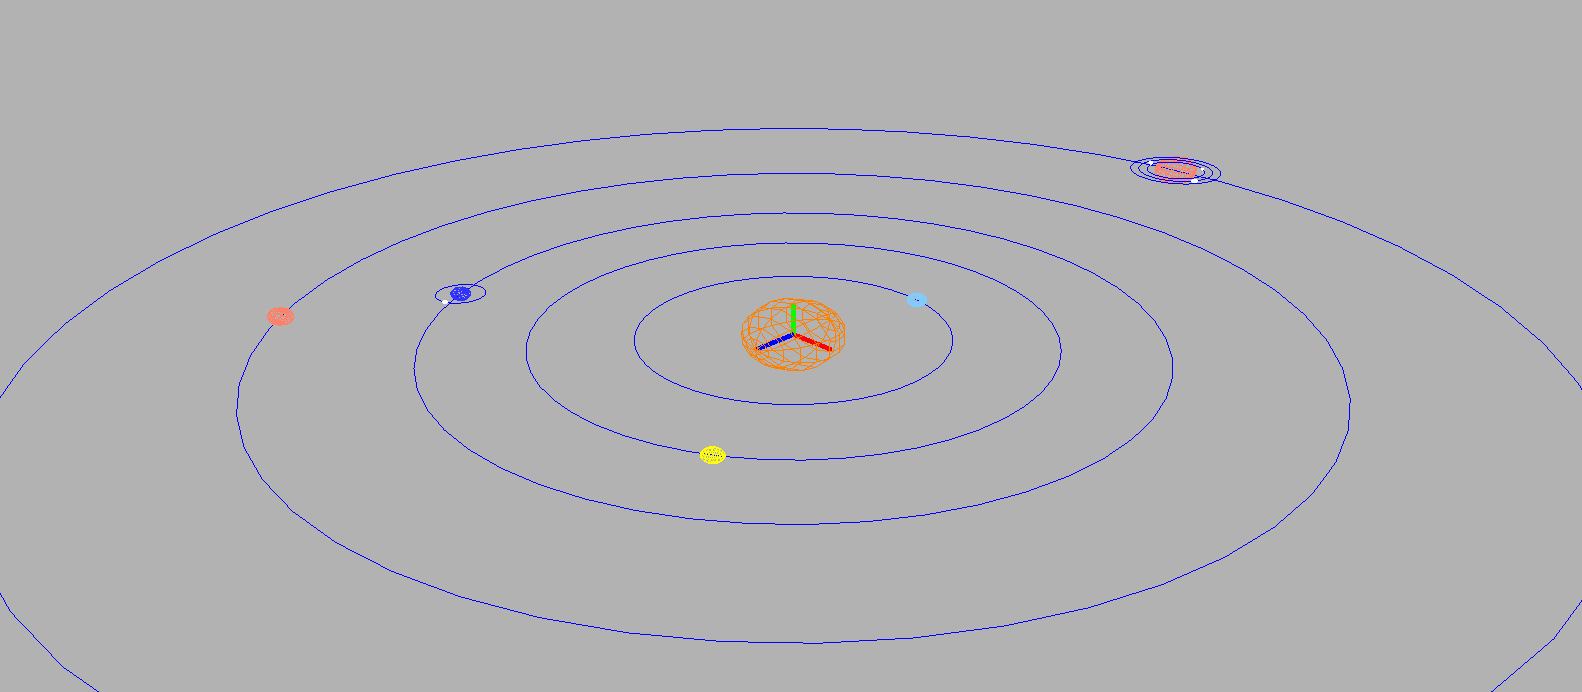
\includegraphics[height=5cm]{OGL_transform/solar2.png}
\end{figure}

\end{frame}
%%%%%%%%%%%%%%%%%%%%%%%%%%%%%%%%%%%%%%%%%%%%%%%%%%%%%%%%%

\end{document}




